%-------------------------------------------------------------------------------
%-------------------------------------------------------------------------------
%-------------------------------------------------------------------------------
\chapter{Révisions}
%-------------------------------------------------------------------------------
%-------------------------------------------------------------------------------
\thispagestyle{empty}
%-------------------------------------------------------------------------------
%-------------------------------------------------------------------------------
\begin{abstract}
Les exercices ici proposés sont classés en fonction de leur niveau de difficulté. Tous les étudiants doivent savoir faire les exercices de niveaux 1 sans problème et parvenir à une solution pour les exercices de niveau 2.
Pour chaque algorithme proposé, on précisera sa complexité en fonction des paramètres fournis.
\end{abstract}
%--------------------------------------------------------------------------
%-------------------------------------------------------------------------------
\section{Niveau 1}
%-------------------------------------------------------------------------------
%-------------------------------------------------------------------------------
\begin{Exercise}Écrire une fonction \type{seuil(x)} telle que
$\displaystyle\text{seuil}(x) = \left\{\begin{matrix} 0&\text{ pour }x \le 0\\
x&\text{ pour }0\le x \le 1\\
1&\text{ pour }1\le x 
\end{matrix}
\right.$
\begin{center}
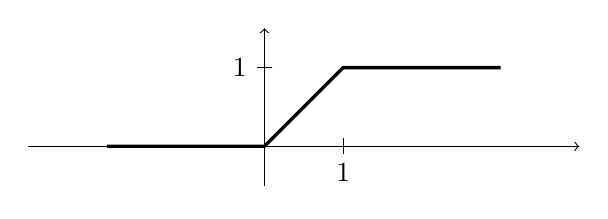
\begin{tikzpicture}
\draw[->] (-3, 0) -- (4, 0);
\draw[->] (0, -0.5) -- (0, 1.5);
\draw (1, 0.1) -- (1, -0.1) node[below] {1};
\draw (0.1, 1) -- (-0.1, 1) node[left] {1};
\draw[very thick] (-2, 0) -- (0, 0) -- (1, 1) -- (3, 1);
\end{tikzpicture}
\end{center}
\end{Exercise}
%-------------------------------------------------------------------------------
\begin{Answer}
\begin{lstlisting}
def seuil(x):
    if x < 0:
        return 0
    elif x < 1:
        return x
    else:
        return 1
\end{lstlisting}
\end{Answer}
%-------------------------------------------------------------------------------
%-------------------------------------------------------------------------------
\begin{Exercise}Écrire une fonction \type{facto(n)} qui calcule $n!$.

En déduire une fonction \type{binomial(n, p)} qui calcule $\binom n p$.
\end{Exercise}
%-------------------------------------------------------------------------------
\begin{Answer}
\begin{lstlisting}
def facto(n):
    f = 1
    for i in range(n):
        f = f*(i+1)
    return f
    
def binomial(n, p):
    return facto(n)//facto(p)//facto(n-p)
\end{lstlisting}
\end{Answer}
%-------------------------------------------------------------------------------
%-------------------------------------------------------------------------------
\begin{Exercise}Écrire une fonction \type{u(n)} qui calcule le terme $u_n$ de la suite définie par $u_0=1$ et $\displaystyle u_{p+1} = \frac{u_p+2}{u_p+1}$ pour $p\in \N$.
\end{Exercise}
%-------------------------------------------------------------------------------
\begin{Answer}
\begin{lstlisting}
def u(n):
    x = 1
    for i in range(n):
        x = (2 + x)/(1 + x)
    return x
\end{lstlisting}
\end{Answer}
%-------------------------------------------------------------------------------
%-------------------------------------------------------------------------------
\begin{Exercise}Proposer une fonction \type{testPres(L, x) } qui teste la présence de l'élément $x$ dans la liste $L$. 
Exemple :  \type{testPres([1,2,27,3],-7) -> False.}
\end{Exercise}
%-------------------------------------------------------------------------------
\begin{Answer}
\begin{lstlisting}
def testPres(L,x):
    n=len(L)
    for k in range(n):
        if L[k] == x:
            return True
    return False 
\end{lstlisting}
\end{Answer}
%-------------------------------------------------------------------------------
\newpage
%-------------------------------------------------------------------------------
\begin{Exercise}
Écrire une fonction \type{maxPerso(L)} qui retourne le maximum de la liste $L$ sans utiliser la fonction max de python.

Écrire une fonction \type{IndiceMax(L)} qui retourne un indice du maximum de la liste $L$.
\end{Exercise}
%-------------------------------------------------------------------------------
\begin{Answer}
\begin{lstlisting}
def maxPerso(L):
    indice=0
    max = L[0]
    for j in range(1, len(L)):
        if L[j]> L[indice]:
            indice = j
            max = L[j]
    return max
\end{lstlisting}

\newpage

L'indice est en fait plus simple, on n'a pas besoin de garder le maximum.
\begin{lstlisting}
def IndiceMax(L):
    indice=0
    for j in range(1,len(L)):
        if L[j]> L[indice]:
            indice = j
    return indice
\end{lstlisting}
\end{Answer}
%-------------------------------------------------------------------------------
\medskip
%-------------------------------------------------------------------------------
{\it On rappelle que l'opérateur \type{\%} calcule le reste de la division (entière), il permet de tester la divisibilité : $p$ divise $n$ si et seulement si \type{n \% p == 0}.}
%-------------------------------------------------------------------------------
%-------------------------------------------------------------------------------
\begin{Exercise}Proposer une fonction \type{testPrime}  qui teste si un nombre fourni en paramètre
est premier.

Exemple :  \type{testPrime(47) -> True}
\end{Exercise}
%-------------------------------------------------------------------------------
\begin{Answer}
\begin{lstlisting}
def testPrime(n):
    k = 2
    while k*k <= n:
        if n%k == 0:
            return False
        k = k+1
    return(True)
\end{lstlisting}
\end{Answer}
%-------------------------------------------------------------------------------
%-------------------------------------------------------------------------------
\begin{Exercise}
Proposer une fonction \type{pgcd(n, p)} qui détermine le plus grand diviseur commun de $n$ et $p$ entiers positifs, c'est-à-dire le plus grand entier qui divise $n$ et $p$. Il est compris entre 1 et \type{min(n, p)}.
\end{Exercise}
%-------------------------------------------------------------------------------
\begin{Answer}
\begin{lstlisting}
def pgcd(a,b):
    commun = 1
    for k in range(1, min(a,b)+1):
        if (a % k == 0) and (b % k == 0 ):
            commun = k
    return commun
\end{lstlisting}
\end{Answer}
%-------------------------------------------------------------------------------
%-------------------------------------------------------------------------------
\begin{Exercise}
Écrire une fonction \type{est\_croissante(liste)} qui renvoie \type{True} ou \type{False} selon que la liste est croissante ou non.
\end{Exercise}
%-------------------------------------------------------------------------------
\begin{Answer}
\begin{lstlisting}
def est_croissante(liste):
    n = len(liste)
    out = True
    for i in range(n-k-1):
        if liste[i+1] < liste[i]:
            out = False
    return out
\end{lstlisting}

Si on veut s'arrêter le plus tôt possible
\begin{lstlisting}
def est_croissante(liste):
    n = len(liste)
    i = 0
    while i < n-1 and liste[i] <= liste[i+1]:
        i = i + 1
    return i == n - 1
\end{lstlisting}
\end{Answer}
%-------------------------------------------------------------------------------
%-------------------------------------------------------------------------------
\section{Niveau 2}
%-------------------------------------------------------------------------------
%-------------------------------------------------------------------------------
\begin{Exercise}
On considère une suite récurrente linéaire d'ordre trois donnée par : $u_0 , u_1 , u_2$ puis la relation $$u_{n+3}=au_{n+2}+bu_{n+1}+cu_n$$. Proposer une fonction qui prenant en paramètres
$u_0,u_1,u_2,a,b,c,n$ retourne $u_n $.

 Exemple: \type{suiteRec(1,2,3,1,1,1,3) -> 6.}
\end{Exercise}
%-------------------------------------------------------------------------------
\begin{Answer}
\begin{lstlisting}
def suiteRec(u0, u1, u2, a, b, c, n):
    v0, v1, v2 = u0, u1, u2
    for k in range(n):
        temp= a*v2 + b*v1 + c*v0
        v0 = v1
        v1 = v2
        v2 = temp
    return v0
\end{lstlisting}
\end{Answer}
%-------------------------------------------------------------------------------
%-------------------------------------------------------------------------------
\begin{Exercise}
Proposer une fonction permettant d'obtenir l'écriture en base 2 de tout nombre entier positif (sous forme de liste de 0 et de 1), puis proposer une fonction réciproque. 

On mettra la liste sous forme des puissances de 2 croissantes c'est-à-dire que $L=[a_0,...,a_{k-1}]$ représente $n=  a_{0}+ 2 a_1 + 4a_2...+2^{k-2} a_{k-2}+ 2^{k-1}a_{k-1}$.

Exemple : \type{ base10To2(13) ->[1, 0, 1, 1] ; base2To10([1, 0, 0, 1, 1]) -> 25}
\end{Exercise}
%-------------------------------------------------------------------------------
\begin{Answer}
\begin{lstlisting}
def base10To2(n):
    nb = n
    liste = []
    while nb > 0:
        liste.append(nb%2)
        nb = nb//2
    return liste
    
def base2to10(L):
    nb = 0
    n = len(L)
    for k in range(n):
        nb = nb + (2**k)*L[k]
    return nb
\end{lstlisting}
\end{Answer}
%-------------------------------------------------------------------------------
%-------------------------------------------------------------------------------
\begin{Exercise}
Déterminer tous les triplets pythagoriciens $[a,b,c]$ tels que $a$ et $b$ sont des entiers de $[\![1,100]\!]$ tels que  $a\le b$ et $a^2 +b^2 =c^2$.

{\it Réponse : il y en a 63}.
\end{Exercise}
%-------------------------------------------------------------------------------
\begin{Answer}
\begin{lstlisting}
def testCarre(n):
    racine = int(n**0.5)
    return (racine**2 == n, racine)
    
def triplet():
    Liste=[]
    for a in range(1,100):
        for b in range(a,100):
            (booleen, racine) = testCarre(a*a+b*b)
            if  booleen:
                Liste.append([a,b,racine])
    return(Liste)
\end{lstlisting}
\end{Answer}
%-------------------------------------------------------------------------------
%-------------------------------------------------------------------------------
\begin{Exercise}
En utilisant la propriété $\binom n p = \frac np \binom {n-1}{p-1}$ pour $1\le p \le n$ et la valeur $\binom n0=1$, écrire une fonction \type{binom(n, p)} qui calcule $\binom n p$ en ne faisant que $p$ multiplication et $p$ divisions entières.
\end{Exercise}
%-------------------------------------------------------------------------------
\begin{Answer}
\begin{lstlisting}
def binom(n, p):
    b = 1
    for i in range(p):
        b = b*(n-p+i+i)//(i+1)
    return b
\end{lstlisting}
\end{Answer}
%-------------------------------------------------------------------------------
%-------------------------------------------------------------------------------
\begin{Exercise}[label = exo:inv]
Proposer une fonction renvoyant une nouvelle liste obtenue en retournant une liste $L$ fournie en paramètre. 
Exemple : \type{inverse([2,4,7,13]) -> [13,7,4,2].}

Proposer ensuite une procédure réalisant cela ``sur place''.

\end{Exercise}
%-------------------------------------------------------------------------------
\begin{Answer}
\begin{lstlisting}
def inverse(L):
    n=len(L)
    miroir =[]
    for k in range(n):
        miroir.append(L[-k-1])
    return miroir
\end{lstlisting}

\newpage

\begin{lstlisting}
def inverseSurPlace(L):
    '''L est modifie après appel a la fonction'''
    n=len(L)
    k=0
    while k<n-k-1:
        temp=L[k]
        L[k] = L[-k-1]
        L[n-k-1] = temp
        k=k+1
\end{lstlisting}
\end{Answer}
%-------------------------------------------------------------------------------
%-------------------------------------------------------------------------------
\begin{Exercise}
Écrire une fonction \type{DeuxMax(L)} qui retourne les deux plus grandes valeurs de la liste $L$ supposées sans doublon.
\end{Exercise}
%-------------------------------------------------------------------------------
\begin{Answer}
\begin{lstlisting}
def DeuxMax(L):
    '''indice1 contient l'indice du max et indice2 contient l'indice du 2e max'''
    if L[0] <L[1]:
        indice1=1
        indice2=0
    else:
        indice1=0
        indice2=1
    for k in range(2,len(L)):
        if L[k]>L[indice1]:
            indice2=indice1
            indice1=k  
        elif L[k]>L[indice2 ]: # dans ce cas L[indice2]<L[k]<L[indice1]
            indice2=k
    return (L[indice2], L[indice1])
\end{lstlisting}
\end{Answer}
%-------------------------------------------------------------------------------
\newpage
%-------------------------------------------------------------------------------
\begin{Exercise}
%-------------------------------------------------------------------------------
\begin{minipage}{0.45\textwidth}
\vspace{0pt}
L'algorithme d'Euclide permet de calculer le PGCD rapidement. Son principe est symbolisé dans le schéma ci-joint.

Expliciter les valeurs de $a$ et $b$ après un passage lorsque, au départ de la boucle, on a $b>a$.

Avec cette méthode, écrire une fonction \type{Euclide(a,b)} qui retourne le PGCD des entiers naturels $a$ et $b$.
\end{minipage}
\hskip 8mm
%-------------------------------------------------------------------------------
\begin{minipage}{0.50\textwidth}
\vspace{0pt}
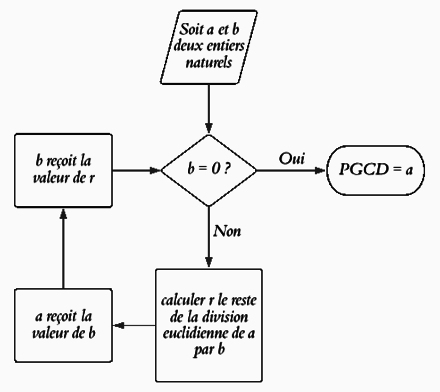
\includegraphics[scale=0.4]{Rev_Euclide}
\end{minipage}
%-------------------------------------------------------------------------------
\end{Exercise}
%-------------------------------------------------------------------------------
\begin{Answer}
\begin{lstlisting}
def Euclide(a, b):
    while b > 0:
        r = a%b
        a = b
        b = r
    return a
\end{lstlisting}
\end{Answer}
%-------------------------------------------------------------------------------
%-------------------------------------------------------------------------------
\begin{Exercise}
Proposer une fonction qui prenant en paramètre une liste contenant au moins deux entiers, détermine les deux éléments les plus proches.  

Exemple : \type{plusProches([2,13,7,15,28]) -> [13,15]}.

Peut-on écrire une fonction plus efficace si on suppose que la liste est triée ?
\end{Exercise}
%-------------------------------------------------------------------------------
\begin{Answer}
\begin{lstlisting}
def plusProches(L):
    n = len(L)
    indice1=0
    indice2=1
    distance = abs(L[1] - L[0])
    for i in range(n):
        for j in range(i+1,n):
            if abs(L[i]-L[j])< distance:
                distance=abs(L[i] - L[j])
                indice1=i
                indice2=j
    return (distance, L[indice1], L[indice2])
\end{lstlisting}
    
La complexité est quadratique, on peut l'améliorer en complexité linéaire si la liste est triée.

\begin{lstlisting}
def plusProches2(L):
    n = len(L)
    indice=0
    distance = abs(L[1] - L[0])
    for i in range(n-1):
        if abs(L[i] - L[1+i])< distance:
                distance=abs(L[i] - L[1+i])
                indice=i
    return (distance, L[indice], L[1+indice])
\end{lstlisting}
\end{Answer}
%-------------------------------------------------------------------------------
%-------------------------------------------------------------------------------
\begin{Exercise}
Écrire une fonction \type{est\_modale(liste)} qui renvoie \type{True} ou \type{False} selon que la liste est modale ou non. Une liste \type{l} est modale s'il existe $p$ compris entre 0 et $n$ ($n$ est sa longueur) telle que \type{l[ : p]} est strictement croissante et \type{l[p :p]} est strictement décroissante ; pour $p=0$ (resp. $p=n$) cela signifie que la liste est strictement décroissante (resp. strictement croissante).
\end{Exercise}
%-------------------------------------------------------------------------------
\begin{Answer}
\begin{lstlisting}
def est_modale(liste):
    n = len(liste)
    i = 0
    while i < n-1 and liste[i] < liste[i+1]:
        i = i + 1
    while i < n-1 and liste[i] > liste[i+1]:
        i = i + 1
    return i == n - 1
\end{lstlisting}
\end{Answer} 
%-------------------------------------------------------------------------------
%-------------------------------------------------------------------------------
\section{Niveau 3}
%-------------------------------------------------------------------------------
%-------------------------------------------------------------------------------
\begin{Exercise}
Proposer une fonction \type{ testPresDicho(L,x)} qui teste la présence de l'élément $x$ dans la liste \underline{triée dans l'ordre croissant} $L$, en procédant à  une dichotomie.
\end{Exercise}
%-------------------------------------------------------------------------------
\begin{Answer}
\begin{lstlisting}
def dicho(L,x):
    '''teste la presence de x dans L'''
    i = 0
    j = len(L)    
    while i < j:      # recherche dans L[i:j] (tranche non vide)
        m = (i+j)//2  # indice du milieu de tranche
        if L[m] == x:
            return True
        if x < L[m]:
            j = m     # recherche dans la partie basse de la tranche
        else:
            i = m + 1 # recherche dans la partie haute de la tranche
    # en sortie i >= j donc la tranche L[i:j] est vide
    return False
\end{lstlisting}
\end{Answer}
%-------------------------------------------------------------------------------
%-------------------------------------------------------------------------------
\begin{Exercise}
Proposer une fonction qui calcule les coefficients binomiaux en utilisant le triangle dit de Pascal. 

Pour calculer $\binom n p$ on calculera la liste des $\binom m k$, $k$ variant de 0 à $m$,  pas-à-pas pour les entiers  $m$ allant de 0 à $n$. 
\end{Exercise}
%-------------------------------------------------------------------------------
\begin{Answer}
\begin{lstlisting}
def binom(n,p):
    liste=[1,1] # pour n=1
    for k in range(n-1): # ici liste est celle de k+1 
        listeTemp = [1]
        for j in range(len(liste)-1):
            listeTemp.append(liste[j]+liste[j+1])
        liste=listeTemp
        liste.append(1)# ici liste est celle de k+2
    return liste[p]
\end{lstlisting}

\newpage

On peut n'utiliser qu'une seule liste.
\begin{lstlisting}
def binom(n,p):
    liste=[1]*(n+1)
    for m in range(n): on calcule les k parmi m
        for k in range(k-1, 0, -1):
            liste[k] = liste[k] + liste[k-1]
    return liste[p]
\end{lstlisting}
\end{Answer}
%-------------------------------------------------------------------------------
%-------------------------------------------------------------------------------
\begin{Exercise}
Une liste $L$ de booléens représente les résultats successifs d'une expérience de Bernoulli. Proposer une fonction qui détermine les longueurs des suites de succès consécutifs. 

Exemple : \type{listeSucces([False,True,True,True,False,True,True]) -> [3,2]}
\end{Exercise}
%-------------------------------------------------------------------------------
\begin{Answer}
\begin{lstlisting}
def listeSucces(L):
    liste = []
    lg = 0
    for k in range(len(L)):
        if L[k]:
            lg = lg + 1
        else:
            if lg > 0:
                liste.append(lg)
                lg = 0
    if lg > 0:
        liste.append(lg)
    return liste
\end{lstlisting}
\end{Answer}
%-------------------------------------------------------------------------------
%-------------------------------------------------------------------------------
\begin{Exercise}
Une application de l'ensemble $[\![1, n]\!]$ dans l'ensemble $[\![1, p]\!]$ est modélisée par la donnée de l'entier $p$ ainsi que la liste ordonnée des images des éléments de $[\![1, n]\!]$.\\
Proposer deux fonctions déterminant si une telle application est injective, puis surjective. 

Exemple : \type{testInj(5,[1,3]) -> True ; testSurj(3,[1,3,1]) -> False.}
\end{Exercise}
%-------------------------------------------------------------------------------
\begin{Answer}
\begin{lstlisting}
def testInj(n,p,L):
    arrivee = [False]*(p+1) # la valeur d'indice 0 ne compte pas
    for y in L:
        if arrivee[y]:
            return False   # la valeur y est deja une image
        arrivee[y] = True  # desormais y est une image
    return True
\end{lstlisting}
    
\begin{lstlisting}
def testSurj(n,p,L):
    arrivee = [False]*(p+1)
    for y in L:
        arrivee[y]=True # desormais  y est connue comme image
    for k in range(1,len(arrivee)):
        if not(arrivee[k]):
            return False # k n'a pas d'antecedent
    return True
\end{lstlisting}
\newpage
\end{Answer}
%-------------------------------------------------------------------------------
%-------------------------------------------------------------------------------
\begin{Exercise}[label = exo:ch3]
Proposer une fonction qui détermine si un nombre est égal à la somme des cubes de ses chiffres. 

Trouver les entiers égaux à la somme des cubes de leurs chiffres (toutes les solutions ont 3 chiffres).
\end{Exercise}
%-------------------------------------------------------------------------------
\begin{Answer}
\begin{lstlisting}
def listeChiffres(n):
    nb = n 
    liste = []
    while nb >0:
        liste.append(nb % 10)
        nb = nb//10
    return liste

def sommeCube(L):
    s = 0
    for x in L:
        s = x**3 + s
    return s

def testCube(n):
    return n == sommeCube(listeChiffre(n))

def cherche():
    for k in range(2, 1000):
        if testCube(k):
            print(k)
\end{lstlisting}
\end{Answer}
%-------------------------------------------------------------------------------
%-------------------------------------------------------------------------------
\begin{Exercise}
Définir une fonction qui, prenant en paramètre un entier $n$, retourne le $n$-ième nombre entier positif supérieur à 10 dont l'écriture en base 10 est symétrique.
\end{Exercise}
%-------------------------------------------------------------------------------
\begin{Answer} Exercice \ref{exo:ch3} pour \type{listeChiffres}, exercice \ref{exo:inv} pour \type{inverse}.
\begin{lstlisting}
def est_miroir(n):
    chf = listeChiffres(n) 
    fhc = inverse(chf)
    return chf == fhc

def sym(n):
    compteur=0
    k=10
    while compteur < n:
        k=k+1
        if est_miroir(k):
            compteur = compteur + 1
    return k
\end{lstlisting}
\end{Answer}
%-------------------------------------------------------------------------------
%-------------------------------------------------------------------------------
\begin{Exercise}[title = {Mines-Ponts 2018}] Une liste $Lalt$ modélise la liste des altitudes d'une succession de points sur un chemin. Proposer une fonction qui retourne les hauteurs des dénivelés successifs des montées et des descentes.

Exemple : {\tt listeDeniveles([0,2,7,13,12,7,15,22,21,25,37]) -> [13,-6,15,-1,16].}
\end{Exercise}
%-------------------------------------------------------------------------------
\begin{Answer}
\begin{lstlisting}
def listeDeniveles(L):
    liste=[]
    n=len(L)
    signe = L[1] - L[0]
    indiceDebut = 0
    for k in range(2, n):
        if signe*(L[k]-L[k-1]) < 0: 
            signe =-signe
            liste.append(L[k-1]-L[indiceDebut])
            indiceDebut = k-1
    liste.append(L[n-1]-L[indiceDebut])
    return liste
\end{lstlisting}
\end{Answer}
%-------------------------------------------------------------------------------
%-------------------------------------------------------------------------------
\begin{Exercise}[label=exo:crible]
Proposer une fonction qui détermine la liste de nombres premiers inférieurs ou égaux à un entier $n$ fourni en paramètre, en utilisant la méthode du crible d'Eratosthène. 

Exemple : \type{crible(22) -> [2,3,5,7,11,13,17,19]}
\end{Exercise}
%-------------------------------------------------------------------------------
\begin{Answer}
\begin{lstlisting}
def crible(n):
    tableau=[True]*(n+1) # l'indice 0 sera inutile
    for k in range(2, n+1):
        if tableau[k]:
            indice = 2*k
            while indice <= n:
                tableau[indice] = False
                indice = indice+k
    liste=[k for k in range(2, n+1) if tableau[k]]
    return liste
\end{lstlisting}
\end{Answer}
%-------------------------------------------------------------------------------
%-------------------------------------------------------------------------------
\begin{Exercise}
Écrire une fonction \type{goldbach(n)} qui retourne un couple de nombres premiers $(a,b)$ tels que $a+b=n$ lorsque $n$ pair. %On pourra utiliser l'exercice \ref{exo:crible}

Exemple  :  \type{goldbach(232) -> (3, 229)} et \type{goldbach(252) -> (11, 241)}

Tester la conjecture selon laquelle tout entier pair supérieur à trois est la somme de deux nombres premiers, jusque 10.000.000 (Conjecture de Golbach). 
\end{Exercise}
%-------------------------------------------------------------------------------
\begin{Answer}
\begin{lstlisting}
def goldbach(n):
    liste = crible(n)
    for j in liste:
        if n-j in liste:
            return j,n-j
\end{lstlisting}
\end{Answer}
%-------------------------------------------------------------------------------
%-------------------------------------------------------------------------------
\begin{Exercise}
On fixe $n$, un entier supérieur à 100. 
Tester sur les nombres $p$ premiers inférieurs à 100 le petit théorème de Fermat : si $p$ ne divise pas $n$, alors  l'entier $ n^{p-1}-1$ est divisible par $p$.
\end{Exercise}
%--------------------------------------------------------------------------
\begin{Answer}
\begin{lstlisting}
def testFermat(n):
    Liste = []
    for k in range(2,100):
        if testPrime(k):
            Liste.append(k)
    for p in Liste:
        if (n%p != 0):
            if not((n**(p-1)-1)% p ==0):
                return False
    return True

\end{lstlisting}
\end{Answer}
%-------------------------------------------------------------------------------
%-------------------------------------------------------------------------------
%-------------------------------------------------------------------------------
\section{Niveau 4}
%-------------------------------------------------------------------------------
%-------------------------------------------------------------------------------
\begin{Exercise}
Proposer une fonction qui détermine si un nombre $n$ fournis en paramètre peut s'écrire comme la somme de cubes d'entiers strictement supérieurs à  1. 

On pourra introduire une matrice de booléens $B$ telles que $B[i,j]$ vaut vrai si et seulement si  $i$ est somme de $j$ cubes d'entiers strictement supérieurs à 1.

Exemple : \type{testSommeCubes(24) -> True}
\end{Exercise}
%-------------------------------------------------------------------------------
\begin{Answer}
\begin{lstlisting}
def sommeCubes(n):
    somme3 = [False]*(n+1)
    somme3[0] = True
    for i in range(1, n+1):
        k = 2
        while k**3 <= i:
            somme3[i] = somme3[i] or somme3[i - k**3]
            k = k + 1
    return somme3[n]
\end{lstlisting}
\newpage
\end{Answer}
%-------------------------------------------------------------------------------
%-------------------------------------------------------------------------------
\begin{Exercise}
On se donne un entier $n$ et trois entiers $a< b<c$ non nuls. écrire une fonction qui donne le nombre de listes à valeurs dans $\{a,b,c\}$ dont la somme des termes vaut $n$. Par exemple, les 7 listes $[1,1,1,1], [1,1,2],[1,2,1], [2,1,1], [2,2],[1,3],[3,1]$ sont à dénombrer lors de l'appel à {\tt nbrSommes(4,[1,2,3])}.
\end{Exercise}
%-------------------------------------------------------------------------------
\begin{Answer}
\begin{lstlisting}
def nbrSommesIter(n,L):
    [a,b,c]=L
    import numpy as np
    B=np.zeros((n+1,n+1),int)
    B[a][1]=1
    B[b][1]=1
    B[c][1]=1
    for j in range(2,n+1):
        for i in range(a,n+1):
            B[i][j] =   B[max(0,i-a)][j-1]
                      + B[max(0,i-b)][j-1]
                      + B[max(0,i-c)][j-1]
    return sum(B[n]) 
\end{lstlisting}
\end{Answer}
%-------------------------------------------------------------------------------
%-------------------------------------------------------------------------------
\begin{Exercise}
On appelle permutation de l'ensemble $[\![1, n]\!]$ une bijection de cet ensemble dans lui-même. Proposer une fonction qui, prenant en paramètre $n$, retourne la liste des
permutations de l'ensemble $[\![1, n]\!]$.

Exemple : {\tt listePerm(3) -> [[1,2,3],[1,3,2],[2,1,3],[2,3,1],[3,1,2],[3,2,1]]}
\end{Exercise}
%-------------------------------------------------------------------------------
\begin{Answer}
\begin{lstlisting}
from copy import deepcopy

def listePerm(n):
    liste=[[1]]
    for k in range(2,n+1):
        newL = []
        for permutation in liste:
            for j in range(len(permutation)+1):
                newL.append(  permutation[:j]
                            + [k]
                            + permutation[j:])
        liste = deepcopy(newL)
    return liste
\end{lstlisting}
\end{Answer}
%-------------------------------------------------------------------------------
%-------------------------------------------------------------------------------
\begin{Exercise}[title = {Exercice des olympiade US, USACO}]
La plupart des sujets des Usaco relatent les aventures de John le fermier et de ses vaches, dont Bessie est la star incontestée.

Bessie suit un régime tel qu'elle ne peut pas manger plus de $C$ $(10\le C\le 35000)$ calories par jour. John le fermier la taquine en plaçant $B$ $(1\le  B\le 21)$ seaux de fourrage, chacun ayant un nombre (pas nécessairement unique) de calories (dans l'intervalle $[\![1,35000]\!])$. Bessie ne sait pas se contr\^oler : une fois qu'elle commence à manger le contenu d'un seau, elle mange tout ce qu'il contient.

Bessie n'est pas très douée pour la combinatoire. Déterminer la combinaison optimale de seaux de fourrage qui donne à Bessie autant de calories que possible sans dépasser la limite $C$.

Par exemple, considérer une limite de 40 calories et 6 seaux de dimensions 7, 13, 17, 19, 29 et 31. Bessie peut manger $7+31=38$ calories mais peut en manger encore plus en consommant trois seaux $7+13+19=39$ calories. Elle ne peut pas trouver de meilleure combinaison.
\end{Exercise}
%-------------------------------------------------------------------------------
\begin{Answer}
\begin{lstlisting}
def bessie(CalMax, nbSeaux, Lprime):
    L = [0] + Lprime 
    L.sort() 
    B=np.zeros((1+nbSeaux, 1+CalMax))
    for p in range(1, 1+CalMax):
        if L[1] <= p:
            B[1][p] = L[1]
    for k in range(1+nbSeaux):
        for p in range(1,1+CalMax):
            if p<L[k]:
                B[k][p] = B[k-1][p]
            else:
                B[k][p] = max(B[k-1][p], B[k-1][p-L[k]]+L[k])
    return B[nbSeaux][CalMax]
\end{lstlisting}
\end{Answer}
%-------------------------------------------------------------------------------
%-------------------------------------------------------------------------------
%-------------------------------------------------------------------------------
